\thispagestyle{formato-PI}
\renewcommand{\MayorVer}{2}
\renewcommand{\MenorVer}{1}
\renewcommand{\FechaPub}{2023--01}
\renewcommand{\TipoID}{PRO}
\renewcommand{\Titulo}{Inspección en la recepción de alimentos}

\section{\Titulo}\index{Inspección!en la recepción de alimentos}
\renewcommand{\Codigo}{\Prog--\thesection--\TipoID}

% \linenumbers

\subsection{Objetivo}
\begin{itemize}
	\item \textbf{Establecer} un programa satisfactorio que asegure que la unidad de transporte se encuentra en condiciones adecuadas de mantenimiento, limpieza y temperatura apropiadas para el almacenamiento dentro de \gls{RDF}
\end{itemize}

\subsection{Alcance}
\begin{itemize}
	\item Este procedimiento aplica para todas las unidades con alimento alimenticio recibidas en RDF;\@
	\item se extiende este documento al área de embarques, pero no se limita a otras áreas operativas.
\end{itemize}

\subsection{Términos y definiciones}
\begin{description}
	\defglo{alimento}
	\defglo{criterio-de-acción}
	\defglo{peligro-relacionado-con-la-inocuidad-de-los-alimentos}
\end{description}

\subsection{Documentos y/o normas relacionadas}
\begin{itemize}
	\item Programa de \glsfirst{BPD}.
\end{itemize}

\subsection{Procedimiento}\index{Procedimiento!inspección en la recepción de alimentos}

\subsubsection{Materiales}
\begin{itemize}
	\item Termómetro IR;\@
	\item Linterna;\@
	\item \Oent.
\end{itemize}

\subsubsection{Precauciones de seguridad}

\begin{itemize}
	\item Usar \emph{uniforme completo.}
\end{itemize}

\subsubsection{Instrucciones de trabajo}
\paragraph{Inspección física de la unidad de transporte}\label{sec:IsnpeccionTransporte}\index{Instrucción!inspección fisica de los alimentos}
\begin{enumerate}
    \item Se verifica la documentación:\\
    Se verifica que cuente con los siguientes documentos:
        \begin{enumerate}
            \item Documentos TIF;\footnote{En caso de ser alimentos de procedencia TIF.}
            \item Listado de alimentos con cantidades;
            \item Especificaciones de almacenamiento del alimento.
        \end{enumerate}

    \begin{itemize}
        \nocumple Se debe de dar aviso al supervisor del almacén para determinar que acciones se pueden tomar;
    \end{itemize}
    
    \item Se verifica la \emph{temperatura programada} de la unidad:\\
    La temperatura programada de la caja debe de coincidir con las especificaciones de almacenamiento del alimento.
    
          \begin{itemize}
            \nocumple Se verifica si la unidad cuenta con un termoregistrador que permita determinar si la temperatura de transporte fué la adecuada, en caso de que no lo tenga, se debe de dar aviso al supervisor del almacén para determinar que acciones se pueden tomar;
          \end{itemize}

    \item Se revisa que el número de sello coincida con la guía y en caso de ser alimento TIF, que el fleje esté intacto:
    \begin{itemize}
        \nocumple Si se descubre que el sello está roto a la llegada, no se puede descargar el alimento y el \emph{Supervisor de Almacén (y/o médico TIF)} debe(n) ser contactado(s) inmediatamente para obtener instrucciones adicionales;
    \end{itemize}
        
        \begin{itemize}
            \item[\textbf{Nota}] Una carga con sello roto puede ser descargada si la misma es un alimento TIF y fue inspeccionada por alguna organización gubernamental y se tiene evidencia de esto.
        \end{itemize}

    \item Se \textit{enrampa} la unidad para descargar el alimento;
    
    \item Inspeccionar la condicion de la caja de transporte:\\
    Se tiene que inspeccionar la condicion de la caja de transporte, prestanto atencion a los siguientes criterios:
    \begin{enumerate}
        \item Limpieza:\\    
        No debe de haber basura y/o escombros que puedan llegar a ocmprometer la inocuidad del alimento.

        \item Evidencia de plagas:\\
        Cualquier presencia de escretas o de plagas visibles son motivo para el rechazo de la unidad.
        
        \item Daño físico a la unidad que comprometa la inocuidad del alimento:\\
        La unidad no puede tener claros por los que pueda ingresar materia del exterior de la caja.

        \item Evidencia de violación de los materiales de empaque:\\
        En caso de encontrar alimento violado, se tiene que verificar si no se hizo una inspección previamente por algún organismo autorizado; de caso contrario, se informará al cliente y el supervisor del almacen determinará las acciones a llevar acabo. 

        \item Presencia de olores extraños:\\
        Es importante reportar olores químicos, como olor a solvente o a plaguicida.
    \end{enumerate}
\end{enumerate}

\begin{scheme}[p]
    \centering
    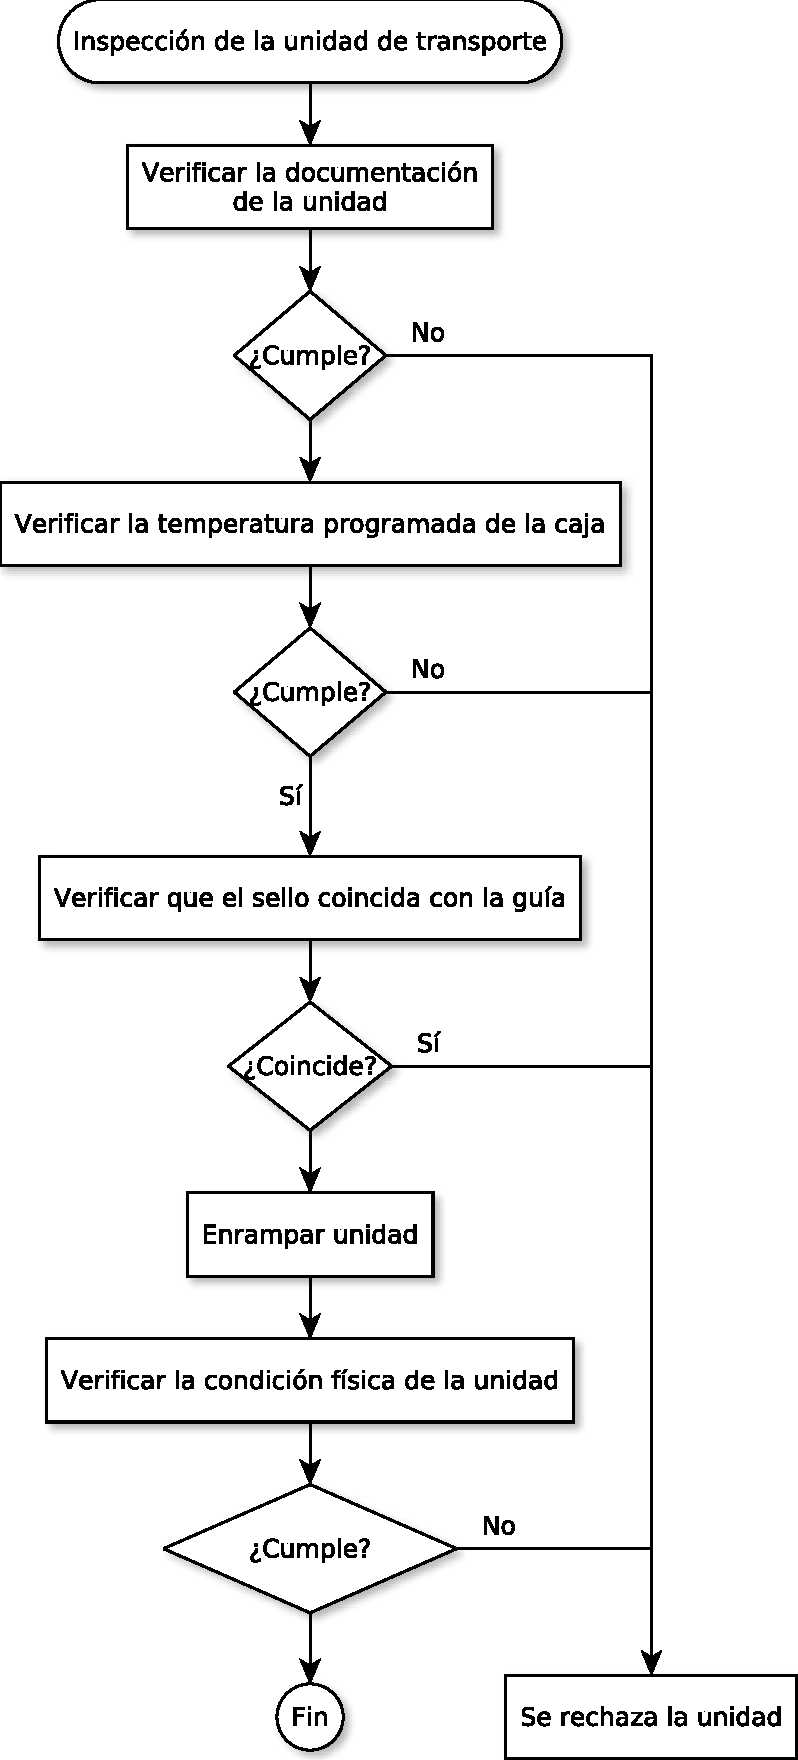
\includegraphics[height=0.9\textheight]{../IT/IT-1-InspeccionDeUnidades.pdf}
    \caption{Proceso de inspección de unidades de transporte. Para mayor información, consultar el \cref{sec:IsnpeccionTransporte}.}
\end{scheme}

\clearpage

\begin{note}[Criterios de acción para la aceptación de alimentos congelados]\label{criterios:aceptacion-cong}
	Si la temperatura de los alimentos al realizar la inspección de la mercancía para su \emph{ingreso} está fuera del rango establecido en el \cref{esp:generica}, se deben de tomar en cuenta las siguientes consideraciones para su aceptación:

	\begin{longtblr}[%
		label={esp.crit.acep},
		caption={Criterios de acción para la descarga de alimentos al almacén.},
		note{\(\dagger\)} = Se tiene que contactar al cliente previo a cualquier procedimiento de acondicionamiento. El cliente es responsable de la preservación del alimento en caso de que rechace el servicio de ráfaga.,
		note{\(\ddagger\)} = La aceptación de esta carga está a disposición de la disponibilidad de la ráfaga.
		]{%
		colspec={X[c]X[3,c]},
		width = 0.7\linewidth,
		rowhead = 1
		}
		\toprule
		\textbf{Intervalo}                 & \textbf{Acción}                                                                                                                                                                                                                                                              \\
		\midrule
		\qty{\geq -3}{\degreeCelsius}      & Se rechaza la carga                                                                                                                                                                                                                                                          \\
		\qtyrange{-7}{-4}{\degreeCelsius}  & Se tiene que inspeccionar la carga de manera profunda para descartar cualquier \gls{peligro-relacionado-con-la-inocuidad-de-los-alimentos} y posteriormente se tiene que enviar a la ráfaga hasta lograr congelar el alimento~\TblrNote{\(\dagger\)}~\TblrNote{\(\ddagger\)} \\
		\qtyrange{-11}{-8}{\degreeCelsius} & Se acepta la carga con cobro adicional por acondicionamiento                                                                                                                                                                                                                 \\
		\qty{\leq -12}{\degreeCelsius}     & Se acepta la carga sin cobro adicional por acondicionamiento                                                                                                                                                                                                                 \\ \bottomrule
	\end{longtblr}
\end{note}

\todo{Hacer la misma tabla para alimentos refrigerados}


\begin{note}[Sobre las temperaturas de los alimentos en la recepción]
	Es importante mencionar que las temperaturas obtenidas al llegar los alimentos al almacén son registradas con un \emph{termómetro infrarrojo (IR),} este en realidad nos arroja la \emph{temperatura superficial del objeto} que vayamos a medir, por lo que \emph{la temperatura \textbf{puede ser mayor} a la de los criterios de aceptación} para la recepción de alimentos, los rangos de temperatura de almacenamiento estan descritos en \cref{esp:generica}, a continuación se detallan de forma resumida:
	\begin{itemize}
		\item Para \emph{alimentos refrigerados,} \gls{RDF} ha establecido con base en regulaciones gubernamentales el rango de temperatura establecido para el \emph{almacenamiento} de alimentos es de \qtyrange{0}{4}{\degreeCelsius}.
		\item Para \emph{alimentos congelados,} se estableció que la temperatura de almacenamiento debe de ser \qty{\leq -12}{\degreeCelsius}.
	\end{itemize}
\end{note}

\paragraph{Descarga de alimentos de la unidad de transporte}\label{sec:DescargaAlimentos}\index{Instrucción!descarga de alimentos de la unidad de transporte}

\begin{enumerate}
    \item Se hace la inspección de la unidad de transporte previo a comenzar a descargar el alimento;
    \item Se \emph{enrampa} la unidad y se abre la cortina del andén.
    \item Se inspeccionan los alimentos conforme a los criterios establecidos de acuerdo a si son:
        \begin{enumerate}
            \item alimentos congelados (ver \cref{esp.crit.acep-cong});
            \item alimentos refrigerados (ver \cref{esp.crit.acep-refri});
            \item alimentos de almacenamiento especial.
        \end{enumerate}
        \begin{itemize}
            \item[\textbf{Si no cumple}] si la temperatura del alimento excede los criterios establecidos para el tipo de almacenamiento, se rechaza la unidad.
        \end{itemize}
    \item Si el alimento viene sobre tarimas, este se descarga de la unidad y se dispone en el andén para que el \emph{personal de embarques} tome nota de la mercancía que se está descargando para posteriormente ingresarla en el \gls{SGA}.
    \begin{enumerate}
        \item En caso de que el \emph{alimento entarimado} requiera de descopete:\\
        se armarán las tarimas adicionales, cuidando el no mezclar lotes diferentes.
        \item En caso de que las tarimas del \emph{alimento entarimado} esten en malas condiciones:\\
        \begin{enumerate}
            \item Si la tarima se puede cargar sin romperse:
                \begin{itemize}
                    \item Se colocará la tarima en malas condiciones sobre una tarima nueva y se cobrará(n) la(s) empleadas.
                    \item Esta accion tiene que registrarse en el \Oent.
                \end{itemize}
            \item Si la tarima viene en muy malas condiciones o si el cargar la tarima podria significar un \gls{peligro-relacionado-con-la-inocuidad-de-los-alimentos}:
                \begin{itemize}
                    \item Se armará una tarima nueva manualmente
                    \item Esta accion tiene que registrarse en el \Oent.
                    \item Se cobrará por armado de tarima y por venta de tarima.
                \end{itemize}
        \end{enumerate}
    \end{enumerate}
    \item Se etiquetarán las tarimas descargadas:\\
    Posterior al ingreso de los datos al \gls{SGA}, {\itshape\MC} genera las etiquetas correspondientes para las tarimas a almacenar. Estas se deben de poner de manera que sean visibles, entre el material de emplaye.
    \item Se almacenarán los alimentos en la cámara correspondiente.
\end{enumerate}

\begin{scheme}[p]
    \centering
    % \missingfigure[figheight=0.9\textheight]{Diagrama sobre descarga de alimentos}
    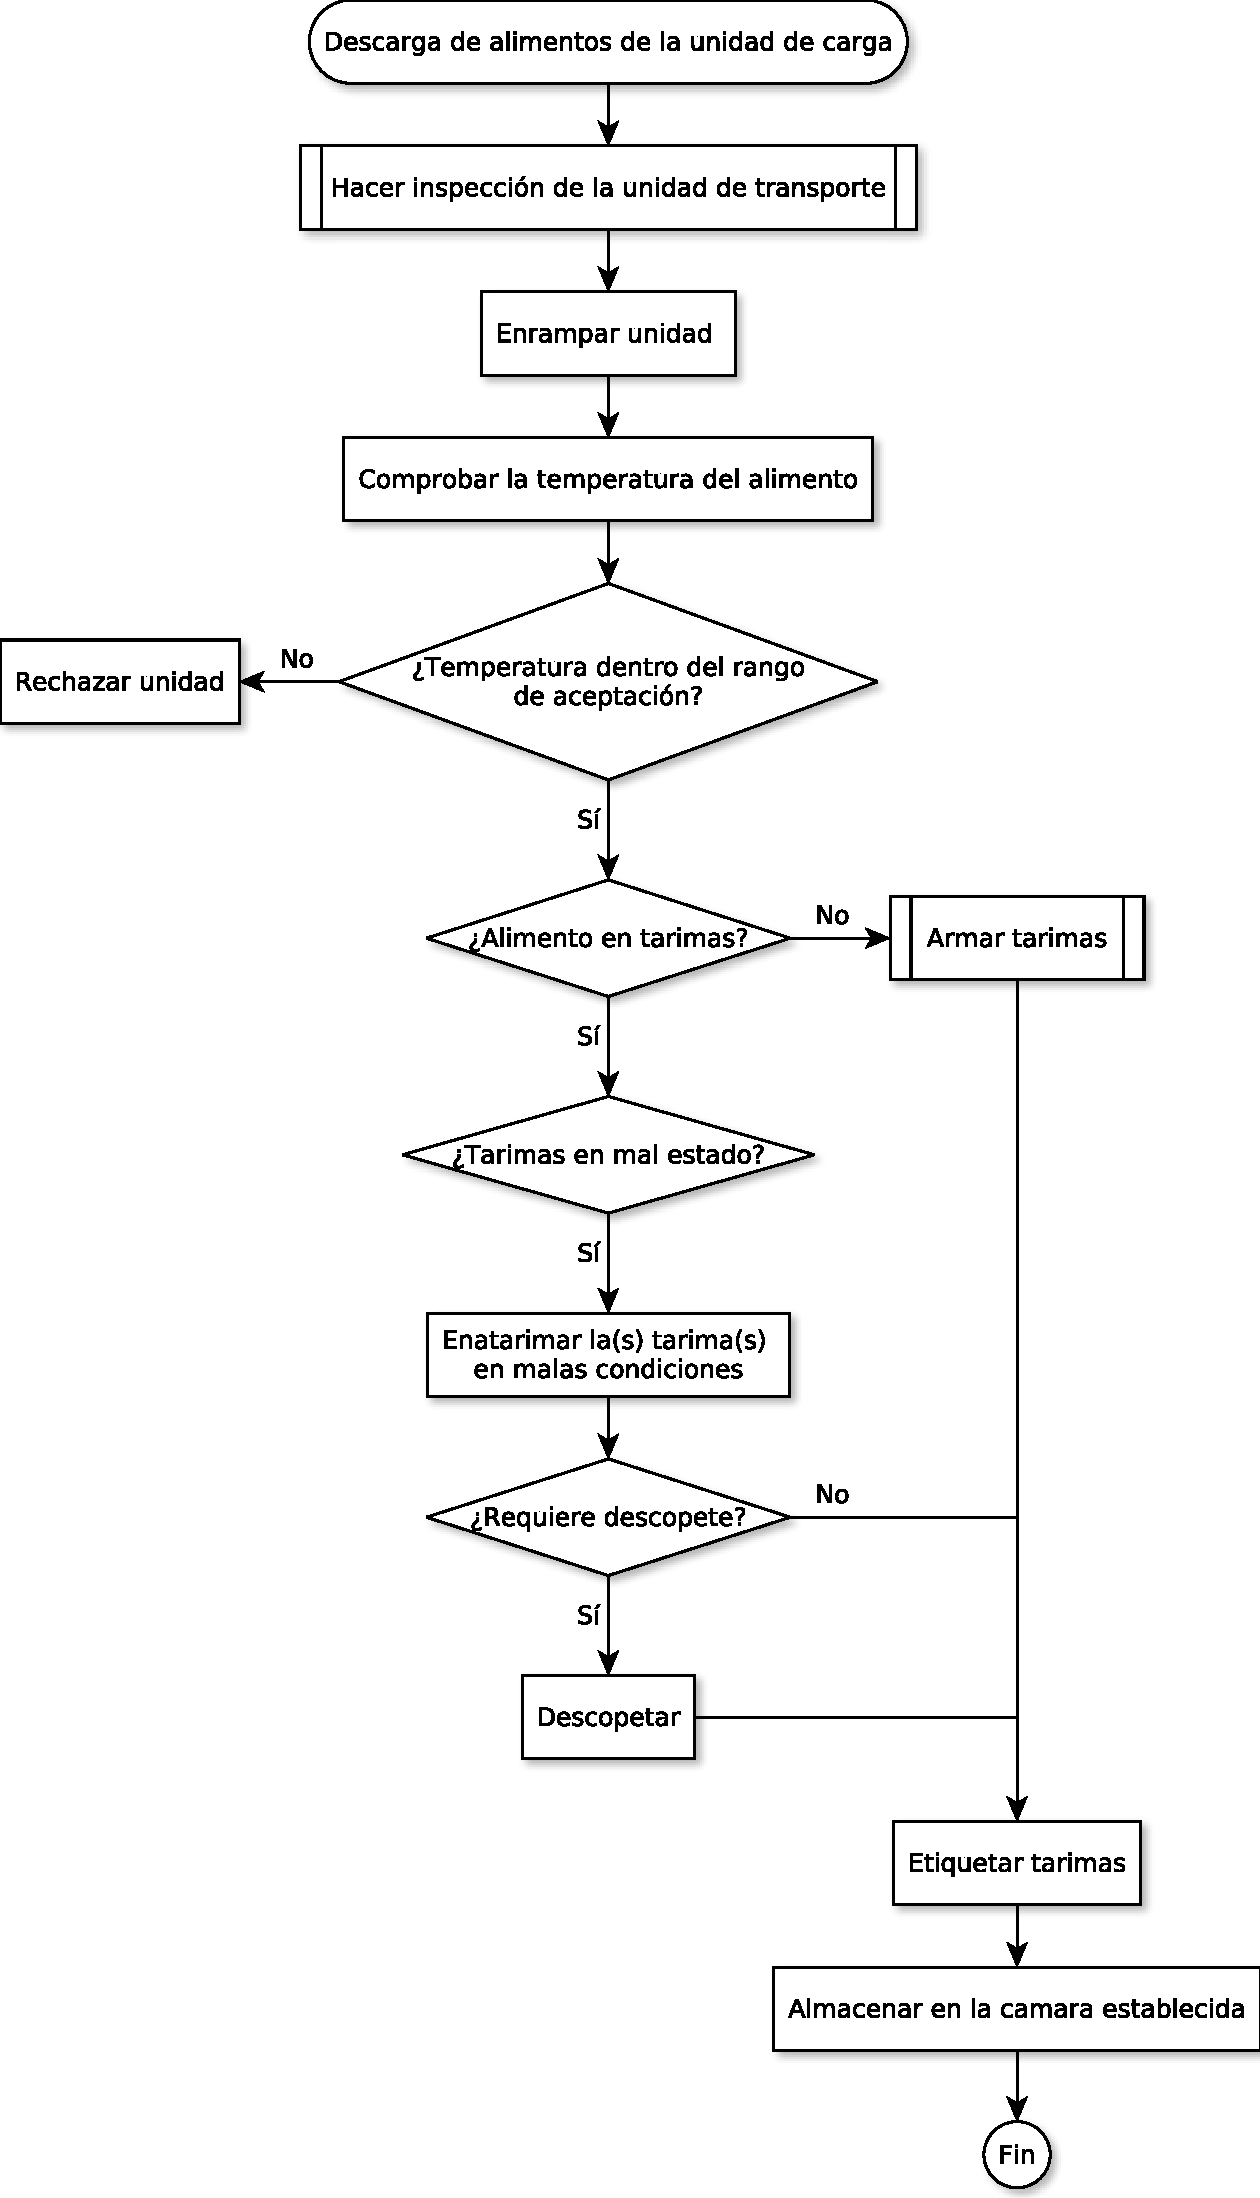
\includegraphics[height=0.9\textheight]{../IT/IT-2.pdf}
    \caption[Proceso de descarga de unidades posterior a la inspección]{Proceso de descarga de unidades posterior a la inspección. Para mayor información, consultar el \cref{sec:DescargaAlimentos}.}
\end{scheme}

\clearpage

\begin{note}[Tiempo máximo de permanencia de alimentos en el andén]\label{TiempoDePermanencia-Anden}\index{Tiempo máximo de permanencia de alimentos en el andén}
	\begin{itemize}
		\item \emph{\textbf{Para alimentos congelados:}} \TiempoAndenCong;
		\item \emph{\textbf{Para alimentos refrigerados:}} \TiempoAndenRefri.
		\item[\textbf{NOTA:}] Este tiempo de permanencia en el andén no aplica para \emph{descargas a granel.}
	\end{itemize}
\end{note}

\subsubsection{Responsables de la actividad}
\begin{itemize}
	\item[\textbf{Ejecutado}] por el personal de operaciones;
	\item[\textbf{Monitoreado}] por personal de aseguramiento de calidad;
	\item[\textbf{Verificado}] por personal de gerencia.
\end{itemize}

\subsubsection{Acciones preventivas}
	Se llevará a cabo una inspección, registrando el indicador y medida correspondiente;
	\begin{enumerate}
		\item \textbf{Si ocurre una insatisfacción:}\\ se capacitará al personal involucrado en ese momento;
		\item \textbf{Si repite una insatisfacción:}\\ si después de la instrucción, se repite la insatisfacción, se tomarán acciones correctivas (\cref{sec:2.1:acc}).
	\end{enumerate}

\subsubsection{Acciones correctivas}\label{sec:2.1:acc}
\begin{itemize}
	\item En caso de no-conformidad, reportar en el formulario de \RAC.
\end{itemize}

\subsubsection{Frecuencia}

Cada recepción de \gls{alimento}.

\begin{changelog}[title=Registro de cambios,simple, sectioncmd=\subsection*]
	\begin{version}[v=2.1, date=2023--07, author=Pablo E. Alanis]
		\item Correcciones a rangos de temperatura;
		\item Reacomodo de las instrucciones de trabajo;
		\item Inclusión de diagrama de flujo del procedimiento.
	\end{version}

	\begin{version}[v=2.0, date=2023--01, author=Pablo E. Alanis]
		\item Cambio de formato;
		\item Cambios en la serialización de versiones;
		\item Se cambió "producto" por "alimento";
		\item Separación entre PPR y PPRO.
	\end{version}
\end{changelog}